\documentclass{beamer}

\usetheme{NapiziaMeeting}
%\usetheme{NapiziaMeetingLite}

\usepackage{graphicx}

%%  %%  %%  %%  %%  %%  %%  %%  %%  %%  %%  %%  %%  %%  %%  %%  %%  %%  %%  %%

\title{Sicilian Translator}
%% \author{Eryk Wdowiak}
\author{\texorpdfstring{Eryk Wdowiak\newline\href{eryk@wdowiak.me}{\texttt{eryk@wdowiak.me}}}{Eryk Wdowiak}}
\institute{Project Napizia}
\date{October 1, 2020}

%\usepackage{hyperref}
\hypersetup{
  %% bookmarks,
  %% bookmarksopen,
  colorlinks=true,
  linkcolor=blue,
  %% citecolor=black,
  %% filecolor=black,
  urlcolor=blue,
  bookmarksnumbered=false,
  pdftitle = {Sicilian Translator},
  pdfauthor = {Eryk Wdowiak},
  %% pdfsubject = {The Quarterly Review of Quarterly Reviews (2020), vol. xx, p. yy-zz},
  %% pdfkeywords = {Sicilian, translation, NLP},
}

%%  %%  %%  %%  %%  %%  %%  %%  %%  %%  %%  %%  %%  %%  %%  %%  %%  %%  %%  %%

\begin{document}

%%  %%  %%  %%  %%  %%  %%  %%  %%  %%

\begin{frame}
  \titlepage
\end{frame}

%%  %%  %%  %%  %%  %%  %%  %%  %%  %%

\begin{frame}
  \frametitle{Why don't we have a Sicilian Translator?}
  \begin{itemize}
    %%
  \item \href{https://translate.google.com/}{Google Translate} doesn't translate Sicilian.
    %%
  \item Nor does \href{https://www.bing.com/translator/}{Bing Translator},
    \href{https://translate.yandex.com/}{Yandex Translate} or
    \href{https://www.deepl.com/translator}{DeepL Translator}.
    %%
  \vspace{1em}
  \item Why not?  And what are we going to do about it?
    %%
  \end{itemize} 
\end{frame}

%%  %%  %%  %%  %%  %%  %%  %%  %%  %%

\begin{frame}
  \frametitle{What is the Sicilian Language?}
  \begin{itemize}
    %%
  \item The Sicilian School of Poets at the imperial court of Frederick II:
    \begin{itemize}
    \item created the first literary standard in Italy (13th century)
    \item inspired Dante, the ``father of the Italian language''
    \end{itemize}
    %%
  \vspace{1em}
  \item Sicilian emerged as a literary language before Italian.
    %%   
  \vspace{1em}
  \item The people of Sicily, Calabria and Puglia speak it everyday.
    \begin{itemize}
    \item They speak Italian at work.
    \item But at home -- with family and friends -- they speak Sicilian.
    \item More precisely, their own dialect of the language.
    \end{itemize}
    %%
  \vspace{1em}
  \item And Sicilian is a language spoken here in Brooklyn, NY.
    %%   
  \end{itemize} 
\end{frame}

%%  %%  %%  %%  %%  %%  %%  %%  %%  %%

\begin{frame}
  \frametitle{So why don't we have a Sicilian Translator?}
  \begin{itemize}
    %%
  \item Because no one had assembled the parallel text to train a translator.
    %%
  \vspace{1em}
  \item It exists! \href{http://www.arbasicula.org/}{Arba Sicula} has been publishing a
    bilingual journal (and many other publications) for over 40 years.
    %%
  \vspace{1em}
  \item So we assembled the parallel text.
    %%
  \end{itemize} 
\end{frame}

%%  %%  %%  %%  %%  %%  %%  %%  %%  %%

\begin{frame}
  \frametitle{Sicilian Translator}
  %% \hspace{-1pt}
  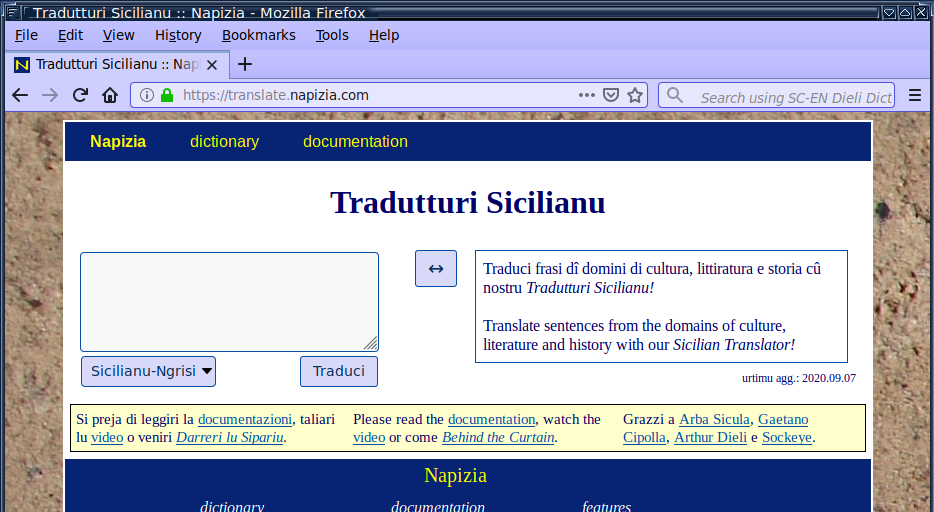
\includegraphics[width=\textwidth]{images/browser-white-box_v1.png}
\end{frame}

%%  %%  %%  %%  %%  %%  %%  %%  %%  %%

\begin{frame}
  \frametitle{How did we do it?}
  \begin{itemize}
    %%
  \item We did \textbf{NOT} start with data collection.
    %%
  \vspace{1em}
  \item We started by collecting the rules of Sicilian vocabulary and grammar.
    \begin{itemize}
    \item Arthur Dieli's \href{http://www.dieli.net/SicilyPage/SicilianLanguage/Vocabulary.html}{\textit{Sicilian Vocabulary}}
    \item Kirk Bonner's \href{http://www.arbasicula.org/LegasOnlineStore.html\#!/28-An-Introduction-to-Sicilian-Grammar-by-J-K-Kirk-Bonner-Edited-by-Gaetano-Cipolla/p/82865123/category=0}{\textit{Introduction to Sicilian Grammar}} (2001)
    \item Gaetano Cipolla's \href{http://www.arbasicula.org/LegasOnlineStore.html\#!/26-Learn-Sicilian-Mparamu-lu-sicilianu-by-Gaetano-Cipolla/p/82865121/category=0}{\textit{Mparamu lu sicilianu}} (2013)
    \end{itemize}
    %%
    \vspace{1em}
    \item And we created the \href{https://www.napizia.com/cgi-bin/cchiu-da-palora.pl}{\textit{Chiù dâ Palora}}
  (\textit{More About the Word}) dictionary.
    \begin{itemize}
    \item vocabulary annotated with grammar, proverbs, poetry, prose and examples
    \item provides a reference for standardizing Sicilian language text
    \end{itemize}
  \end{itemize}
\end{frame}

%%  %%  %%  %%  %%  %%  %%  %%  %%  %%

\begin{frame}
  \frametitle{More About the Word}
  \vspace{-1.25em}
  \begin{center}
    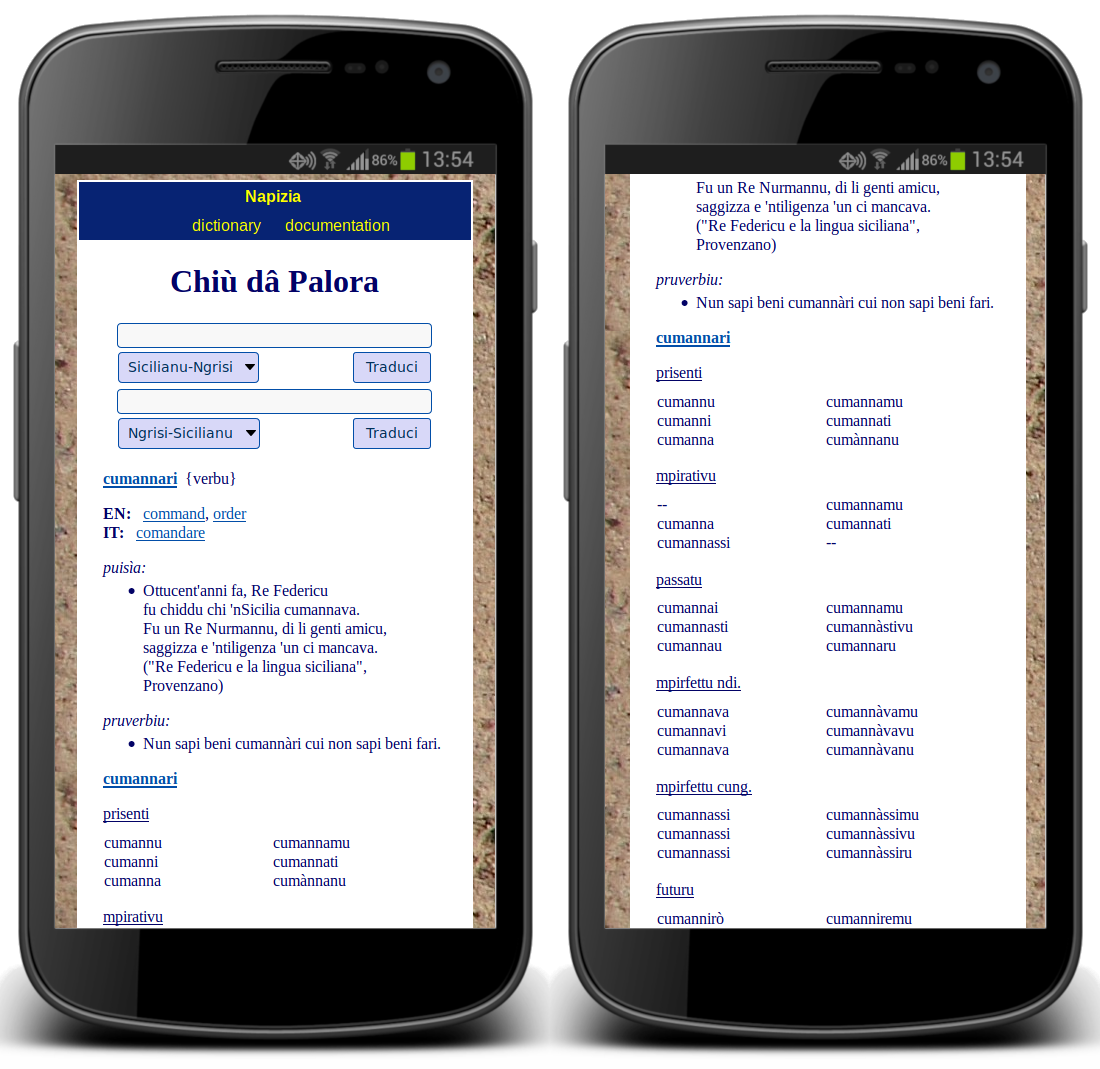
\includegraphics[height=0.795\textheight]{images/cdp_cumannari_v2.png}
  \end{center}
\end{frame}


%%  %%  %%  %%  %%  %%  %%  %%  %%  %%

\begin{frame}
  \frametitle{Then We Began Collecting Data}
  \begin{itemize}
  \item Sources of parallel text:
    \begin{itemize}
    \item the bilingual literary journal \href{https://www.arbasicula.org/}{\textit{Arba Sicula}}
    \item \href{http://www.dieli.net/}{A.~Dieli}'s translations of Sicilian poetry, proverbs and \href{https://en.wikipedia.org/wiki/Giuseppe_Pitr\%C3\%A8}{G.~Pitrè}'s \href{https://scn.wikipedia.org/wiki/F\%C3\%A0uli,_nueddi_e_cunti_pupulari_siciliani}{\textit{Folk Tales}}
    \item examples from G.~Cipolla's \href{http://www.arbasicula.org/LegasOnlineStore.html\#!/26-Learn-Sicilian-Mparamu-lu-sicilianu-by-Gaetano-Cipolla/p/82865121/category=0}{\textit{Mparamu}} and K.~Bonner's \href{http://www.arbasicula.org/LegasOnlineStore.html\#!/28-An-Introduction-to-Sicilian-Grammar-by-J-K-Kirk-Bonner-Edited-by-Gaetano-Cipolla/p/82865123/category=0}{\textit{Introduction}}
   \end{itemize}
  %% \item Textbook examples greatly improved translation quality. (See below).
  \vspace{0.5em}
  \item Data Preparation
    \begin{itemize}
    \item Selected Sicilian language text that could be edited to Standard Sicilian.
    \item Used \href{https://github.com/danielvarga/hunalign}{\textit{hunalign}} to identify translated sentence pairs.
    \item Manually edited the Sicilian language text for quality and standardization.
    \end{itemize}
  \vspace{0.5em}
  \item Our parallel corpus (so far):
    \begin{itemize}
    \item 14,494 lines for training -- 196,911 Sicilian words, 202,652 English words
    \item 121 hand selected for validation -- 1836 Sicilian words, 1878 English words
    \end{itemize}
  \end{itemize} 
\end{frame}

%%  %%  %%  %%  %%  %%  %%  %%  %%  %%

\begin{frame}
  \frametitle{And We Began Modeling}
  \begin{itemize}
  \item We trained our translation models with \href{https://awslabs.github.io/sockeye/}{Sockeye}.
  \vspace{0.25em}
  \item Adding parallel text always improves translation quality more than adjusting hyperparameters.
  \vspace{0.25em}
  \item But some ways of training a model are better than others.
  \vspace{0.25em}
  \item We avoid overfitting by training:
    \begin{itemize}
    \item a self-attentional Transformer model \href{https://arxiv.org/abs/1706.03762}{(Vaswani et al., 2017)}%%,
      %% which directly models the relationships between words in a pair of sentences.
    \item a smaller network with fewer layers \href{https://arxiv.org/abs/1905.11901}{(Sennrich and Zhang, 2019)}
    \item with small subword vocabularies \href{https://arxiv.org/abs/1508.07909}{(Sennrich, Haddow and Birch, 2016)}
    \item with high-dropout parameters \href{http://jmlr.org/papers/v15/srivastava14a.html}{(Srivastava et al., 2014)}
    \end{itemize}
  \vspace{0.25em}
  \item Large empirical improvements when we added theoretical knowledge:
    \begin{itemize}
    \item by pushing the subword splitting toward ``textbook'' desinences
    \item by using textbook examples to give structure to the sequences
    \end{itemize}
  \end{itemize}
\end{frame}

%%  %%  %%  %%  %%  %%  %%  %%  %%  %%

\begin{frame}
  \frametitle{Evaluating the Models}
  \begin{itemize}
  \item Translation quality improves with parallel text.  As our dataset grew
    from 120,000 to 200,000 words, our BLEU scores increased:
    \begin{itemize}
    \item from 11.4 to 22.5 on English-to-Sicilian translation
    \item from 12.9 to 25.2 on Sicilian-to-English translation
    \end{itemize}
  \vspace{0.5em}
  \item Within a given dataset, pushing the subword splitting toward ``textbook'' desinences increased BLEU scores:
    \begin{itemize}
    \item from 20.3 to 22.4 on English-to-Sicilian translation
    \item from 21.4 to 24.1 on Sicilian-to-English translation
    \end{itemize}
  \vspace{0.5em}
  \item We also observed larger increases in BLEU scores when we added parallel text from 
    textbook examples than from other sources.
    \begin{itemize}
    \item We did not conduct any formal tests to confirm this observation.
    \item With our eyes, we could see the structure that textbook examples added.
    \end{itemize}
  \end{itemize} 
\end{frame}

%%  %%  %%  %%  %%  %%  %%  %%  %%  %%

\begin{frame}
  \frametitle{Next Steps}
  \begin{itemize}
  \item We still have more issues of \href{https://www.arbasicula.org/}{\textit{Arba Sicula}} to extract text from.
  \item So we'll add more parallel text and further increase translation quality.
    \vspace{1em}
  \item We may also use the Sicilian text to train word embeddings and create lists of context similar words for our dictionary,
    \href{https://www.napizia.com/cgi-bin/cchiu-da-palora.pl}{\textit{Chiù dâ Palora}}.
    \vspace{1em}
    \item And we'll add more proverbs and poetry to the dictionary too.
  \end{itemize}
\end{frame}

%%  %%  %%  %%  %%  %%  %%  %%  %%  %%

\begin{frame}
  \frametitle{Come to Napizia!}
  \begin{itemize}
  \item So come to \href{https://www.napizia.com/index.shtml}{Napizia} and try our
    \href{https://translate.napizia.com}{\textit{Tradutturi Sicilianu}}\textit{.}
    \vspace{1em}
  \item To see how it works ``behind the curtain,'' come:
    \href{https://translate.napizia.com/cgi-bin/darreri.pl}{\textit{Darreri lu Sipariu}}\textit{.}
    \vspace{1em}
  \item To learn more, please read some of our documentation:
    \begin{itemize}
    \item \href{https://www.napizia.com/pages/sicilian/translator.shtml}{Sicilian Translator} at Napizia
    \item \href{https://www.doviak.net/pages/ml-sicilian/index.shtml}{Introduction to Sicilian NLP}
    \item \href{https://www.doviak.net/pages/ml-sicilian/ml-scn_p05.shtml}{A Recipe for Low-Resource NMT}
    \item \href{https://github.com/ewdowiak/Sicilian_Translator}{Sicilian Translator} at Github
    \end{itemize}
    \vspace{0.5em}
    \item We hope you'll join us.  \textbf{\textit{Grazzi!}}
  \end{itemize}
\end{frame}

%%  %%  %%  %%  %%  %%  %%  %%  %%  %%

\end{document}

%%  %%  %%  %%  %%  %%  %%  %%  %%  %%
% %%  %%  %%  %%  %%  %%  %%  %%  %%
%%  %%  %%  %%  %%  %%  %%  %%  %%  %%

%% \begin{frame}
%%   \frametitle{frame title}
%%   \begin{itemize}
%%   \item text
%%   \item text
%%   \end{itemize} 
%% \end{frame}

%%  %%  %%  %%  %%  %%  %%  %%  %%  %%

%% \hspace{-1pt}
%% 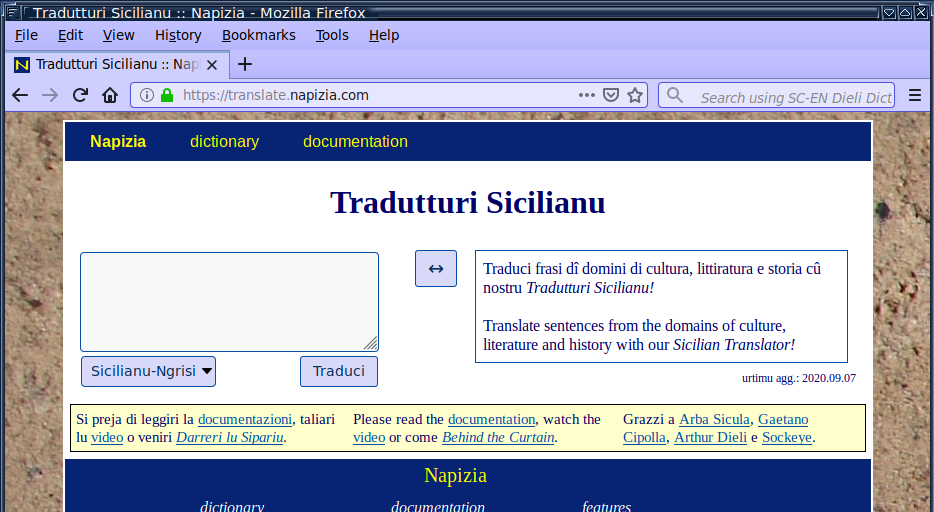
\includegraphics[
%%   %% trim={"left"}{"bottom"}{"right"}{"top"}
%%   trim={0.0in} {0.0in} {0.0in} {0.0in},
%%   clip=true]{images/browser-white-box_v1.png}

%%  %%  %%  %%  %%  %%  %%  %%  %%  %%
